\chapter{Contribuição: StarVZ sobre Spark} \label{ch:contribution}

A fase de pré-processamento do arcabouço StarVZ é similar a um fluxo de Ciência 
de Dados. Nele, são carregadas e manipuladas várias tabelas, utilizando 
bibliotecas do pacote \texttt{tidyverse}. Este Capítulo fala sobre as diferenças 
propostas e realizadas no StarVZ, com o objetivo de otimizar o tempo de 
execução da fase de pré-processamento. Resumidamente, no lugar de tabelas R, 
utilizaremos tabelas Spark (\emph{Spark Dataframes}) para o carregamento e 
manipulação de dados. Na Seção \ref{sect:arch} são apresentadas as mudanças 
arquiteturais propostas e na Seção \ref{sect:implement}, detalha-se a 
implementação dessas mudanças.

\section{Arquitetura Proposta} \label{sect:arch}

A arquitetura da aplicação que este trabalho se propõe a modificar pode ser 
visualizada na Figura \ref{fig:starvz-app}. Os dados, já em formato 
\textit{CSV} são lidos com a biblioteca \texttt{readr}. Com estes em memória, 
são realizadas filtragens e junções com o auxílio das bibliotecas \texttt{dplyr} 
e \texttt{tibble}. Finalmente, os dados são escritos em disco no formato 
\textit{Feather}, usando a biblioteca de mesmo nome. Todo esse processo é 
conduzido através de um código R.

\begin{figure}[ht]
 \centerline{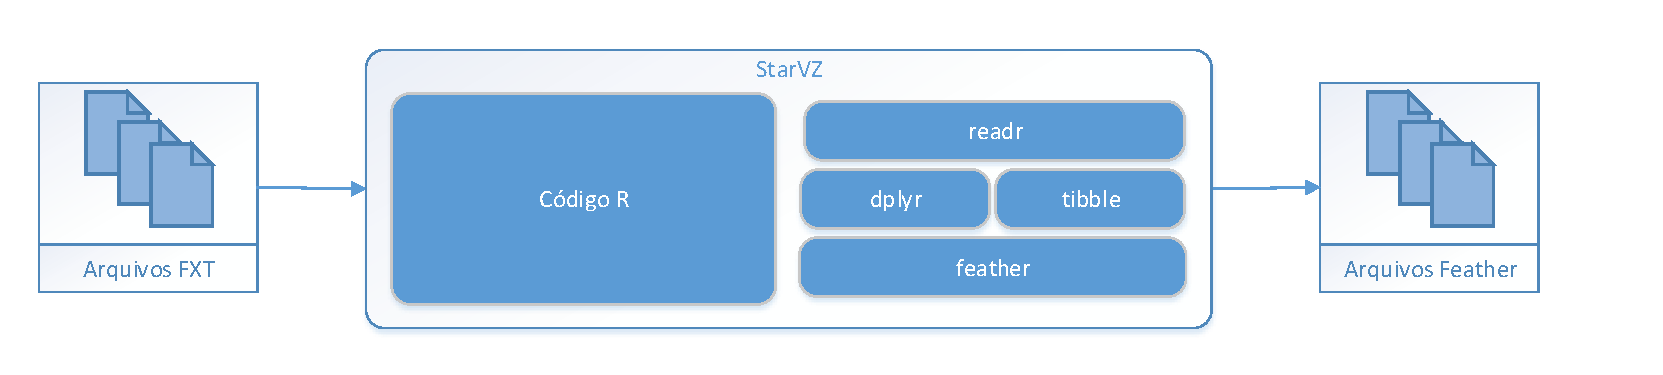
\includegraphics[width=1\textwidth]{./img/starvz-arch.pdf}}
 \caption{Arquitetura da aplicação StarVZ.}
 \label{fig:starvz-app}
\end{figure}

Durante o trabalho, identificou-se que não havia uma biblioteca que suportasse a 
escrita de tabelas Spark em arquivos \textit{Feather}. Isso é essencial para 
compararmos a escrita do mesmo tipo de dados tanto na execução sequencial quanto 
na distribuída. Devido ao ecossistema Hadoop utilizar o formato \textit{Parquet} 
\cite{ref:parquet} como padrão para armazenamento de dados colunares, o fluxo 
sequencial da aplicação foi adaptado para escrever suas saídas neste formato, 
utilizando a biblioteca \texttt{Apache Arrow}.

A Figura \ref{fig:starvz-app-spark} ilustra a arquitetura da aplicação após as 
modificações propostas. Considerando o tamanho dos arquivos de entrada, 
utilizaremos o HDFS para armazená-los. Todavia, o arquivo entities não cresce 
muito com o aumento do tamanho das entradas (seu tamanho fica na ordem de 
KBytes). Para este, o custo de armazená-lo e tratá-lo no sistema de arquivos 
distribuído não é vantajoso pois os processamentos adicionais para realizar tais 
processos são mais caros que o tratamento do arquivo em si. Portanto, decidiu-se 
mantê-lo com seu armazenamento no sistema de arquivos local e processamento 
sequencial.

\begin{figure}[ht]
 \centerline{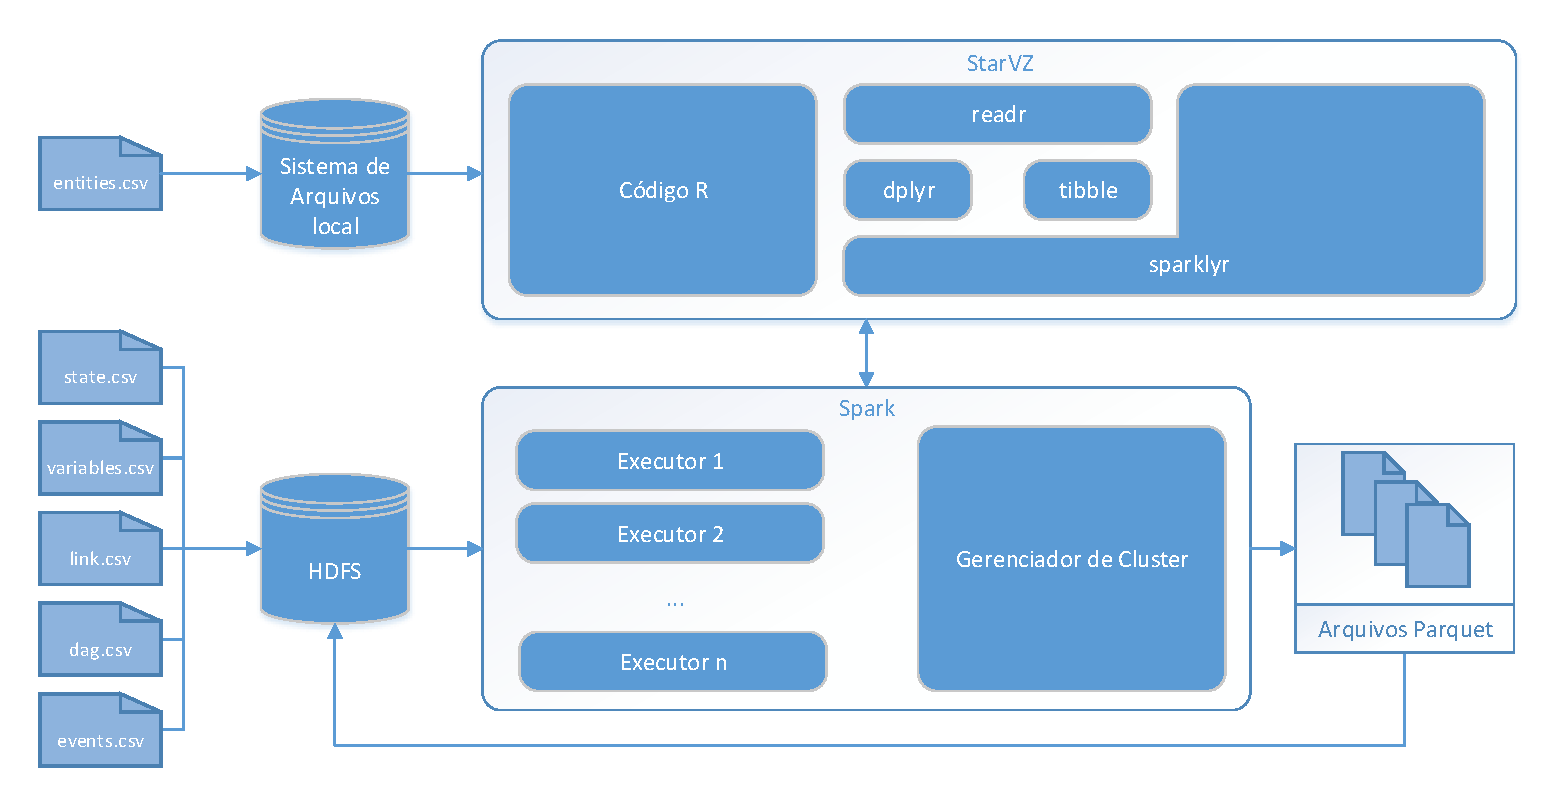
\includegraphics[width=1\textwidth]{./img/starvz-arch-spark.pdf}}
 \caption{Arquitetura da aplicação StarVZ utilizando Spark.}
 \label{fig:starvz-app-spark}
\end{figure}


A biblioteca escolhida para fazer a intermediação entre o código R e o Spark 
foi a \texttt{sparklyr}. De acordo com \citet{ref:sparkbook}, ela é 
baseada no pacote \texttt{dplyr} e sua abordagem prioriza a experiência com R, 
abstraindo alguns dos conceitos básicos como a seção Spark (\emph{Spark 
Session}), diferindo da abordagem padrão das APIs. O processo Driver, 
responsável por intermediar operações no código R e no Spark, é encapsulado nas 
tratativas dessa biblioteca. 

O Spark utiliza diretamente o HDFS para leituras e escritas. Todas as tabelas 
de saída são escritas no HDFS. No caso da tabela Entities, após seu 
processamento ela é convertida em uma tabela Spark. Com isso, padroniza-se o 
local de saída do arcabouço.



\section{Implementação} \label{sect:implement}

Nesta Seção, começaremos dando uma visão geral das modificações realizadas no 
pacote StarVZ. Em seguida, aprofundaremos o fluxo de processamento da aplicação 
original (sequencial) e da modificada (distribuída), mostrando que ambas seguem 
praticamente o mesmo fluxo. Por fim as modificações realizadas são detalhadas e 
a forma que elas foram validadas é explicitada.

A execução do script da fase de pré-processamento agora conta com o parâmetro de 
tipo, onde \texttt{-S}, significa sequencial e \texttt{-D}, distribuído. Este 
foi criado dentro do próprio pacote StarVZ como um novo conjunto de funções, 
permitindo ao usuário a utilização de qualquer metodologia do arcabouço.

A Figura \ref{fig:spark-starvz-flow} representa os possíveis fluxos da 
aplicação.  As formas que possuem o contorno Sequencial e o preenchimento 
Distribuído representam etapas que sempre são executadas. As formas que possuem 
preenchimento meio a meio, representam etapas que contam com uma implementação 
diferente para cada tipo de fluxo, executado conforme parametrizado. As formas 
que possuem apenas um preenchimento correspondem a etapas que são executadas 
sempre com a abordagem preenchida.

\begin{figure}[H]
 \centerline{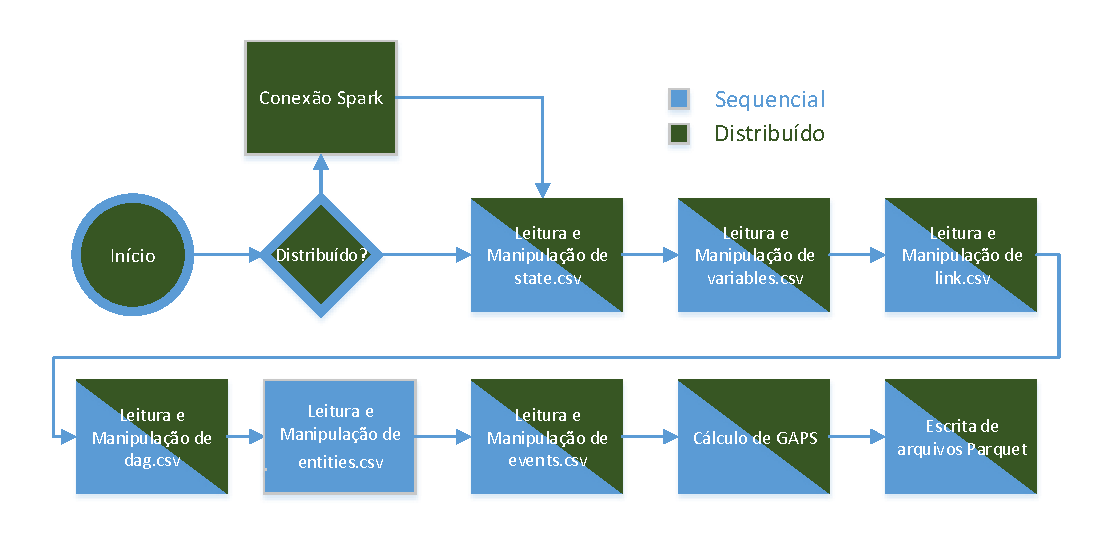
\includegraphics[width=1\textwidth]{./img/applicationflow.pdf}}
 \caption{Fluxo de execução da aplicação.}
 \label{fig:spark-starvz-flow}
\end{figure}

Sobre o fluxo, a única modificação realizada foi a criação da conexão com Spark 
caso o usuário esteja utilizando o arcabouço de forma distribuída. Este 
trabalho teve como objetivo otimizar o processamento dentro de cada 
etapa, apesar de haver margem para a paralelização de operações nesse nível. 
Destaca-se que, conforme mencionado na Seção anterior, o processamento de 
Entities foi mantido sempre no formato sequencial.

No fluxo original, a escrita de arquivos foi modificada para o formato 
\textit{Parquet}, com o pacote \texttt{Apache Arrow}. Em termos de código, essa 
modificação é bastante pontual, adicionando uma importação de biblioteca e 
modificando os métodos de escrita de arquivos (de \texttt{write\_feather} 
para \texttt{write\_parquet}). É importante salientar que este pacote também 
conta com uma implementação de \texttt{write\_feather}, que é mais eficiente 
que aquela do pacote \texttt{feather}.

Para utilizar a \textit{Engine} e executar a aplicação de forma distribuída, é 
necessário estabelecer uma conexão Spark, utilizando o método 
\texttt{spark\_connect}. Com ela estabelecida, é possível ler arquivos em 
diversos formatos diretamente para tabelas no \texttt{sparklyr}. Esse processo 
é realizado na etapa de Conexão Spark, executada em caso de fluxo distribuído 
conforme representado na Figura \ref{fig:spark-starvz-flow}.É importante 
ressaltar que com essa biblioteca, conseguimos ler arquivos armazenados no HDFS, 
o que permite que volumes de dados maiores que a quantidade de memória 
disponível na máquina sejam processados. Essa funcionalidade é muito importante 
pois desvincula o potencial da aplicação da limitação física da infraestrutura 
utilizada.

Com os arquivos carregados em tabelas Spark o restante do trabalho 
foi identificar equivalências entre as transformações realizadas com 
\mytexttt{dplyr} na \mytexttt{sparklyr}. Como esta foi desenvolvida baseada na 
primeira, esse processo foi facilitado. Ao encontrar uma manipulação, o seu 
resultado era observado na tabela original e reproduzido com funções suportadas 
pela \texttt{sparklyr}. Essa metodologia foi adotada pois, caso fosse necessário 
um tratamento que não fosse suportado pela biblioteca, seria preciso 
implementá-lo via funções definidas pelos usuários (\emph{User defined function 
ou UDFs}). Essa funcionalidade sofre de problemas de desempenho ao utilizar R ou 
Python pois há o custo de instanciar um processo R e compartilhar os dados de 
entradas e saídas. 

A Tabela \ref{tab:equivalence} exibe as principais equivalências utilizadas. 
As funções adaptadas com elas geraram as versões distribuídas de tratamento de 
todas as tabelas, com exceção de entities que ficou com seu processamento 
sequencial. Enquanto a maior parte das operações possui uma equivalência de um 
pra um, a função \texttt{separate} necessita de um conjunto de transformações 
para chegar no mesmo resultado. 

\begin{table}[H]
\centering
\begin{tabular}{l l} \toprule
\textbf{Operação \texttt{dplyr}}  &  \textbf{Operação \texttt{sparklyr}}\\ 
\midrule
distinct	& unique  \\
sort		& sdf\_sort \\
gsub		& regexp\_replace\\
rbind		& union\_all\\
grepl		& rlike\\
separate	& ft\_regex\_tokenizer + sdf\_separate\_column       \\
\end{tabular}
\caption{Equivalências de operações.}
\label{tab:equivalence}
\end{table}

A última transformação de dados a ser realizada antes da escrita dos arquivos 
\textit{Parquet}, cálculo de GAPS, é um conjunto de junções realizadas 
de forma recursiva. Durante o desenvolvimento, foi observada que a versão 
distribuída levava um tempo maior que a execução sequencial. Isso foi atribuído 
ao custo de comunicação de Executores e aos processamentos que o Spark 
executa dentro desta etapa (lembrando sua execução \emph{Lazy}) e foi um ponto 
de atenção levantado para ser observado durante os experimentos.

Logo após o cálculo de GAPS, os dados estão prontos para serem escritos. Neste 
ponto foi realizada a validação dos resultados, executando ambos os 
fluxos da aplicação com um conjunto de dados de 835 MB. Para cada um, validamos 
tabela por tabela, realizando diversas operações de sumarização e comparando 
seus resultados. Por exemplo, na tabela State, realizamos a comparação do 
número de linhas das tabelas (ambas tinham 5207577 linhas), além da comparação 
de 7 agrupamentos diferentes. A tabela \ref{tab:validation} reproduz os dados 
observados em ambos os fluxos ao realizar-se o agrupamento dos dados pela coluna 
Type.

\begin{table}[H]
\centering
\begin{tabular}{l c} \toprule
\textbf{Agrupamento}  &  \textbf{Número de Linhas} \\ 
\midrule
Communication Thread State	& 199180 \\
Memory Node State		& 326886 \\
Worker State			& 952006 \\
User Thread State		& 1623915 \\
hread State			& 2105590 \\
\end{tabular}
\caption{Número de linhas dos dados da tabela State agrupados pela coluna Type}
\label{tab:validation}
\end{table}

Por fim, as saídas são escritas no HDFS. Elas geram múltiplos arquivos, por 
exemplo, se a saída se chamar \emph{teste.parquet}, a aplicação criará um 
diretório com esse nome e dentro dela haverá diversos arquivos, conforme abaixo. 
Isso ocorre pois por padrão as tabelas Spark são particionadas e escrevê-las 
gera um arquivo por partição.

\footnotesize
\begin{lstlisting}
 part-00000-1c143c87-5361-427c-825e-792497a8fa61-c000.snappy.parquet
 part-00001-1c143c87-5361-427c-825e-792497a8fa61-c000.snappy.parquet
 ...
\end{lstlisting}






